\documentclass[oneside, a4paper, onecolumn, 10pt]{article}

% Change this: Customize the title, author, advisor, abstract
\newcommand{\thesistitle}[0]{Linearization of Concurrent Data Structures}
\newcommand{\authorname}[0]{Mark Daychman}

\newcommand{\supervisor}[0]{Prof. Constantin Enea}
\newcommand{\supervisorinstitution}[0]{LIX \& CNRS}

\newcommand{\abstracttext}[0]{%
Lorem ipsum dolor sit amet, consectetur adipiscing elit, sed do eiusmod tempor incididunt ut labore et dolore magna aliqua. Ut enim ad minim veniam, quis nostrud exercitation ullamco laboris nisi ut aliquip ex ea commodo consequat. Duis aute irure dolor in reprehenderit in voluptate velit esse cillum dolore eu fugiat nulla pariatur. Excepteur sint occaecat cupidatat non proident, sunt in culpa qui officia deserunt mollit anim id est laborum.
}

\usepackage[
  left=2cm,top=2.0cm,bottom=2.0cm,right=2cm,
  headheight=17pt, % as per the warning by fancyhdr
  includehead,includefoot,
  heightrounded, % to avoid spurious underfull messages
]{geometry}

\usepackage{listings}
\usepackage{color}
\usepackage[dvipsnames]{xcolor}

\lstset{
  language=Python,
  basicstyle=\color{black}\ttfamily\footnotesize,
  numberstyle=\color{gray},
  commentstyle=\color{OliveGreen}\bfseries,
  emph={[2]def,from,import,pass,return,try,for,except,in,if,else, elif}, emphstyle={[2]\color{purple} \bfseries},
  emph={[3]exec, values, copy, popFirst, min, append, intersects},emphstyle={[3]\color{BlueViolet} \bfseries},
  showstringspaces=false,
  emph={[4],int, Call, List,Dict, State, True, False}, emphstyle={[4]\color{Orange}\bfseries},
  breaklines=true,
  emph={[5]dfs, linearize_generic, CAS, sort_by_thread}, emphstyle={[5]\color{blue} \bfseries},
  prebreak=\mbox{{\color{gray}\tiny$\searrow$}},
  numbers=left,
  xleftmargin=25pt
}


\lstnewenvironment{python}[1][]
{
\pythonstyle
\lstset{#1}
}
{}


\usepackage[T1]{fontenc}
\usepackage{subfig}
\usepackage{amstext}
\usepackage{amsmath}
\usepackage{amssymb}
\usepackage{url}
\usepackage{graphicx}
\usepackage{wrapfig}
\usepackage{enumerate}
\usepackage{paralist}
\usepackage{xspace}

\usepackage{varwidth}
\usepackage{times}
\usepackage[colorlinks,linkcolor=blue]{hyperref}
\usepackage[colorinlistoftodos,prependcaption,textsize=normal]{todonotes}
\usepackage{pdfpages}
\usepackage{fancyhdr} %% For changing headers and footers

\usepackage{titling}
\usepackage[nottoc,numbib]{tocbibind}

%% \predate{}
%% \postdate{}
%% \date{}
%% \author{\authorname}


\begin{document}

%\title{\thesistitle}

%\maketitle

% Max 10 lines.
%\noindent \paragraph*{Abstract}
%\abstract

\hspace{0pt}
\vfill

\begin{center}


\includegraphics[width=0.3\textwidth]{logo-EP-vertical}

\vspace*{2em}
%
{\large
\textbf{\'Ecole Polytechnique}

\vspace*{1em}
\textit{BACHELOR THESIS IN COMPUTER SCIENCE}


\vspace*{3em}
{\Huge \textbf{\thesistitle}}
\vspace*{3em}



\textit{Author:}

\vspace*{1em}
\authorname{}, \'Ecole Polytechnique

\vspace*{2em}
%
{\textit{Advisor:}}

\vspace*{1em}
\supervisor{}, \supervisorinstitution{}
}

\vspace*{2em}
\textit{Academic year 2022/2023}

\end{center}

\vfill
\hspace{0pt}

\newpage

\vfill
\noindent\textbf{Abstract}\\[1em]
%
\fbox{
\parbox{\textwidth}{
\abstracttext{}
}
}
\vfill


\newpage

% Setting up the header
\pagestyle{fancy}
%\renewcommand{\headrulewidth}{0pt} % Remove line at top
%\renewcommand{\headrulewidth}{0.4pt}% Default \headrulewidth is 0.4pt
\lhead{\authorname}
%\chead{\acronym}
\rhead{\thesistitle}



\newpage
\tableofcontents
\newpage

%\pagenumbering{arabic}

\section{Introduction}

\subsection{Introduction of Concurrency and Consistency Models}

Concurrency is an ability of a system to execute parts of the program in a different order without affecting the final result. These parts can be physically executed at the same time on different cores of a CPU (parallel computing) or they can execute on the same core by, for example, interleaving their execution (concurrent computing), but at all times on one computation takes place. The main goal of concurrent algorithms is to achieve the same result as the sequential algorithm, but in a shorter time. The problem that arise when two concurrently executing threads attempt to communicate and share some common resource. Potential problems include race conditions (when a thread reads a value that is then updated by another thread, rendering all further operations of the first thread invalid) or deadlocks (when two threads are waiting for each other to release a resource). On top of that the number of execution paths in a concurrent program grows exponentially, and the result can be indeterminant.\\\\
The problems that may arise during concurrent calculations motivate the creation of consistency models that specify how different threads can interact with these shared resources to ensure accurate results. One of the fundamental consistency models is sequential consistency. This model informally states that all operations within a single thread or core are executed in the order they appear in the program, but the order of the threads themselves is undefined. The main benefit of sequential consistency is that it provides a simple and intuitive model for understanding the behavior of concurrent programs. The programmer can reason about the program's execution as if it were a single sequential program, which makes it easier to develop and debug concurrent programs. Additionally, sequential consistency ensures that all threads observe the same order of operations, which can prevent errors such as race conditions and deadlocks. However, sequential consistency also has its drawbacks. It can result in significant performance overheads because of the need for synchronization and communication between threads, which can limit parallelism. This can make it difficult to scale concurrent programs to take advantage of multiple processor cores or distributed computing environments. Additionally, the strict ordering of operations required by sequential consistency can limit the flexibility of concurrent program execution, making it more challenging to optimize for performance. \\\\
A stronger consistency model is linearizability, defined by Herlihy and Wing. \cite{HerlihyWing} "Linearizability provides the illusion that each operation applied by concurrent processes takes effect instantaneously at some point between its invocation and its response, implying that the meaning of a concurrent object’s operations can be given by pre- and post-conditions." (Herlihy and Wing, 1987) Two of the greatest advantages of linearizability over a sequential model is that it is compositional and non-blocking. Compositionality means that if linearizability of operations is proved for several programs separately, then the programs together will also be linearizable. In a linearizable program the launched operations do not require other operations to be launched for their termination. This is the property of non-blockability. 
\subsection{Non-blocking Algorithms and Atomic Operations}

There are some classic approaches to combatting the problems of concurrency. One of them is to use locks. Locks are a mechanism for controlling access to a shared resource. A lock can be in one of two states: locked or unlocked. When a thread wants to access a shared resource, it first acquires the lock for that resource and only then reads from or modifies the memory. This prevents other threads from accessing the resource until the lock is released. The main problem with locks is that they can cause a thread to block, waiting for the lock to be released. This can cause a thread to wait indefinitely if another thread holding the lock crashes or is otherwise unable to release it. This is known as a deadlock. Additionally, locks can cause significant performance overheads because of the need for synchronization between threads.
Ideally, we do want our concurrent algorithms to not block when one of the threads fails and never releases the lock. Algorithms that have this property are called non-blocking. With few exceptions, non-blocking algorithms use atomic read-modify-write primitives that the hardware must provide, the most notable of which is compare and swap (CAS).[???] Atomic operations are operations that are guaranteed to be executed atomically by the hardware. This means that the operation will either complete in its entirety or not at all. This property is useful when implementing concurrent algorithms, because without the inefficiency of locks, we can be certain to avoid race conditions. The Python-style pseudocode (which will be used throughout this paper) for an atomic CAS is shown in Figure \ref{Atomic CAS}. Two other most commonly used atomic operations are atomic writes and reads, and some architectures even include more complex operations, such as atomic test-and-set and fetch-and-add, as well as store conditionals.[???] In reality, the mutex locks themselves, as well as other synchronization mechanisms like semaphores are implemented using atomic operations.[???]\\
\begin{figure}
  \centering
  \begin{minipage}{0.65\textwidth}
      \centering
      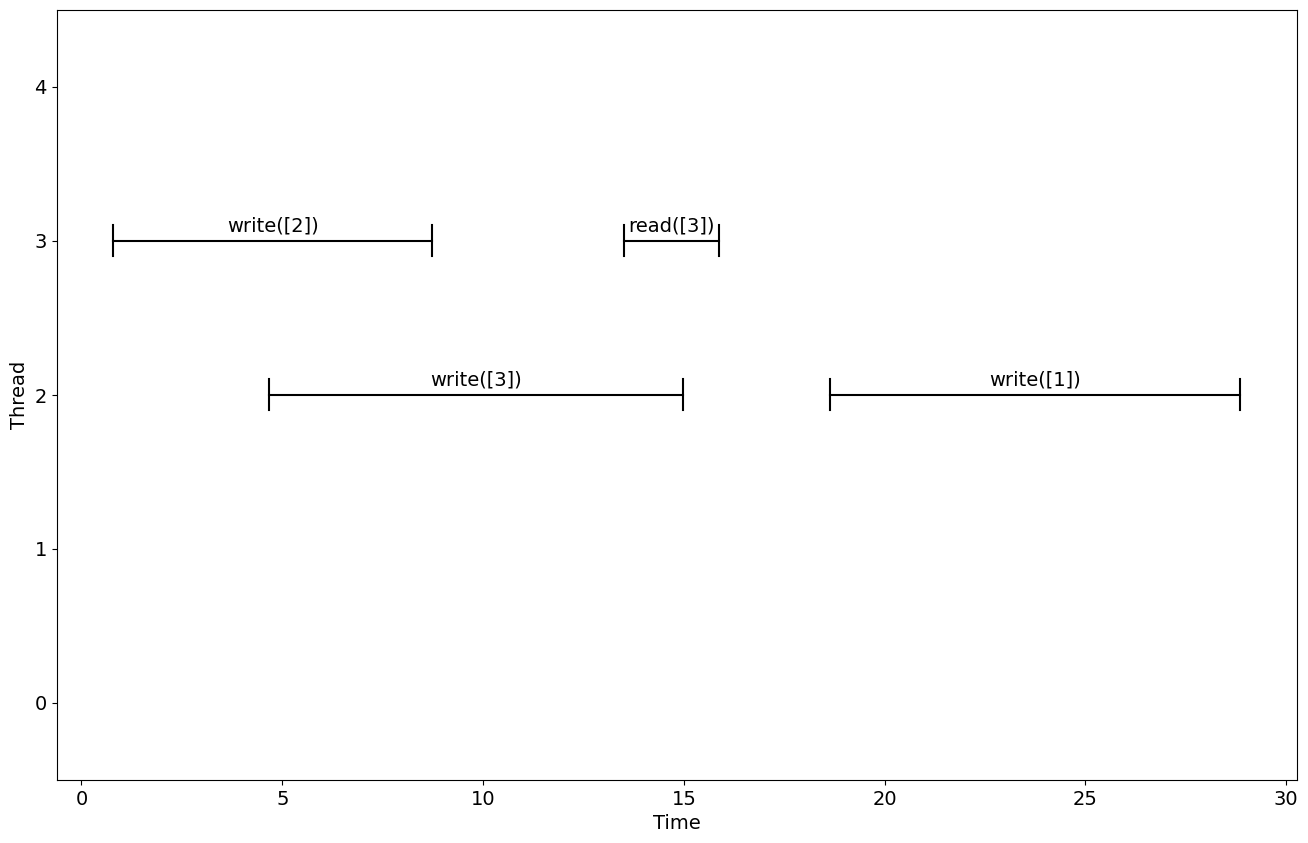
\includegraphics[width=0.9\textwidth]{assets/io_spec_simple.png} 
      \caption{\label{Simple IO history}An example of a 2-thread history}
  \end{minipage}\hfill
  \begin{minipage}{0.3\textwidth}
      \centering
      \begin{lstlisting}[language=Python]
def CAS(x, old, new):
  if x == old:
    x = new
    return True
  else:
    return False
       \end{lstlisting} 
      \caption{\label{Atomic CAS} Atomic CAS pseudocode}
  \end{minipage}
\end{figure}

\section{Checking Linearizability}
\subsection{Problem Introduction}
As stated before, linearizability of a sequential characterization, (also known as a history or a sequential specification), assumes that the effect of an operation takes place instantaneously at some moment between the call of the operation and its return. For simplicity, we can denote the call of that operation or function as an interval in time between its call and return. An example of a specification with 2 threads and 4 operations is given in Figure \ref{Simple IO history}. 
In general, the problem of checking whether a specification is linearizable is NP-complete. [???]. However, for some sets of operations and under certain constraints this problem can be solved in polynomial time. A common example is a concurrent stack with queues and dequeues on unique values (see section \ref{}). In this paper, we will focus on linearizing the following set of operations under the given constraints:
\begin{itemize}
  \item \textbf{State.} The state represents a single shared resource, in our case a single memory cell storing an integer. The initial value of the state is undefined and must be set prior to any reads or compares.
  \item \textbf{Atomic read and write.} Writes set the value of the state to a new value, potentially overriding the value written previously. An important constraint is that writes are unique, meaning a value can only be written to memory once, and that value can never be written again. This constraint may seem excessive, but in reality, we can always apply versioning and use a unique identifier for each write without changing the output of the algorithm. On the other hand, this constraint allows us to reason about some partial order between the variables. There can be multiple reads on the same value, and reads do not in any way alter the state. To linearize a read, we just need to pick a point in time when the value of the state is equal to the value read.
  \item \textbf{True CAS.} Both true and false CASs have two arguments, the first being the value the CAS expects to be in memory and the second being the value to be written to memory if the compare succeeds. True CAS expects the compare to succeed. In a sense, a true CAS is both a read and a write, but the two must come immediately one after another with no operation linearized in between. 
  \item \textbf{False CAS.} A false CAS expects the compare to fail. In this case, the value of the state is not changed. A false CAS is in some sense the opposite of a read, as it can be linearized by all but one value. An additional constraint we put on false CASs is that there is always at least one read that has already returned on the compare value. This constraint arises from the practical uses .....
  \item \textbf{2-state switch.} TBD
\end{itemize}
To linearize a specification means to pick a unique linearization point within the interval of each operation, such that the resulting linearization is a valid execution of the program. For example, in Figure \ref{Simple IO history}, the linearization point of \verb|read(3)| must happen after that of \verb|write(3)|, as otherwise the read fails. Likewise, the intervals of \verb|write(2)| and \verb|write(3)| intersect, but since linearizing \verb|write(2)| after \verb|write(3)| would fail the read, we must linearize it before. Finally, the linearization point of \verb|write(1)| in all cases happens last. This forces a unique linearization: \verb|[write(2)|, \verb|write(3)|, \verb|read(3)|, \verb|write(1)]|. Notice how the location of linearization points forces a certain order of operations, so for simplicity, we will reason about the order of linearization rather than the exact location of the linearization points. Furthermore, the linearization order need not be unique. Figure \ref{Multiple Linearizations} shows an example of a history that has multiple linearizations. Indeed, the reads from threads 1 and 2 can be performed in any order and the linearization will still be valid.\\\\

\begin{figure}
  \centering
  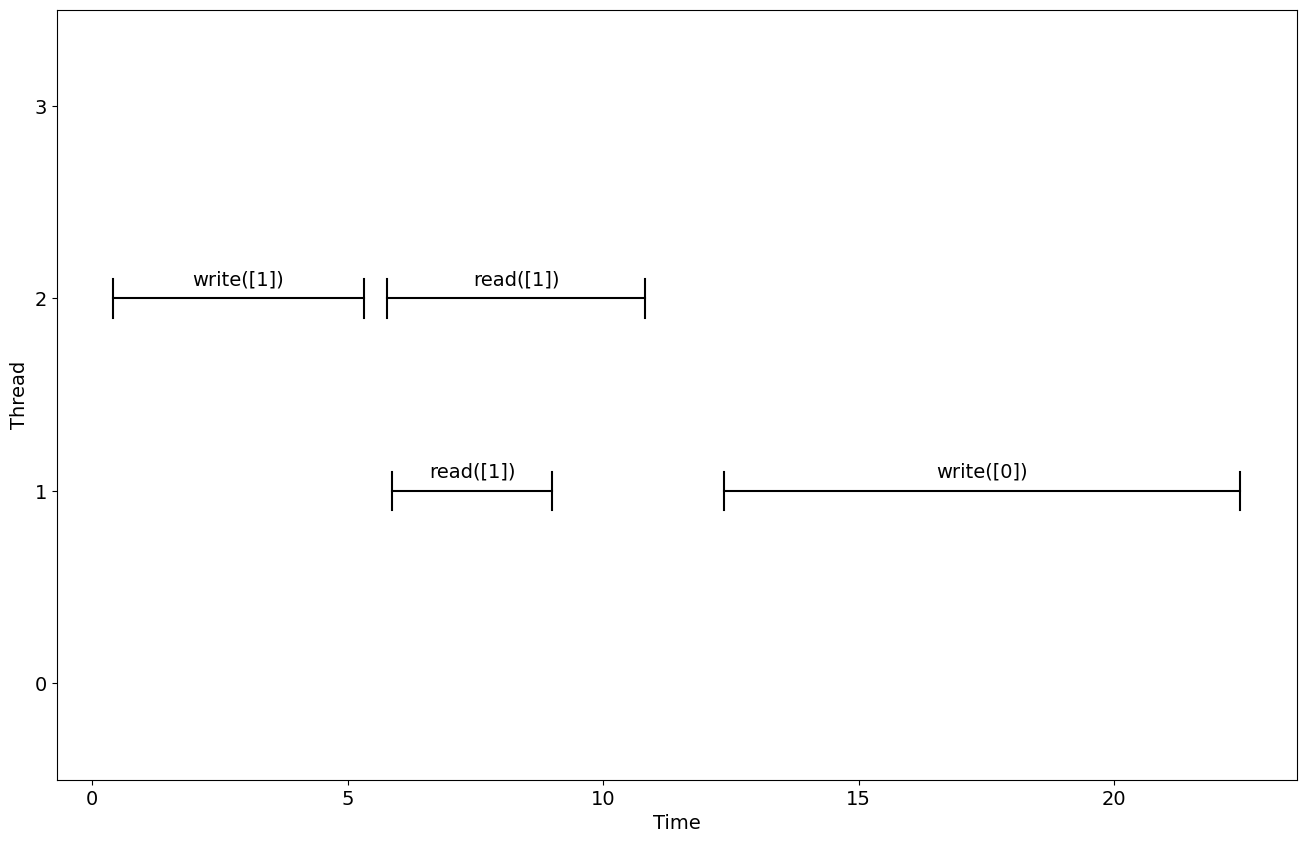
\includegraphics[width=0.7\textwidth]{assets/io_mult_lins.png}
  
  \caption{\label{Multiple Linearizations}A history with multiple linearizations}
  
\end{figure}

\subsection{Brute Force Approach}
The obvious brute force approach to linearize a specification is to try all possible linearizations and check which ones are valid. This approach is obviously infeasible for large specifications, because of the exponential sample space, but it can be used to check small specifications. Programmatically, we sort the operations by thread number and within each thread by the starting point of each operation. We keep track some internal state depending on which kind of operations we are trying to linearize. We begin from the operation that starts the earliest, execute it and then first traverse all operations that intersect the current operation, otherwise if they were all explored, we move on to the next unexplored operation that starts the earliest. If during linearization, the execution throws an error, we backtrack. The pseudocode for the algorithm is given in Figure \ref{Brute-force Linearization Verifier}. 

\begin{figure}
  \begin{center}
    \begin{lstlisting}[language=Python]
      def dfs(threads: Dict[int, List[Call]], state: State):
        res: List[List[Call]] = []
        first_op_per_thread = [t.first for t in threads.values()]
        if first_op_per_thread.isEmpty:
            return res
        ref = min(op.end for op first_op_per_thread)
        # candidates are all the operations we can execute next
        # without violating the linearization order
        candidates: List[Call] = [c in first_op_per_thread if c.intersects(ref)]
      
        for c in candidates:
            try:
                # new execute the operation on a copy of the state
                # and if an execution throws and error, we backtrack
                new_state = c.exec(state.copy())
            except:
                return
      
            sol = dfs(threads.copy()[c.threadno].popFirst(), new_state)
            res.append(sol)
      
        return res
      
      def linearize_generic(spec: List[Call], state: State):
        # sort by thread and then by start time
        threads: Dict[int, List[Call]] = sort_by_thread(spec)
        ret = dfs(threads, state)
      
        return ret
      
          
        \end{lstlisting}
  \end{center}
  \caption{\label{Brute-force Linearization Verifier}Brute-force linearization verifier}
\end{figure}
\subsection{Linearizability of a Concurrent Queue}
\subsection{Linearizability of I/O Operations}
\subsubsection{Atomic Read and Write}
\subsubsection{True CAS}
\subsubsection{False CAS}
\subsubsection{2-state Switch}
\section{Testing}
Tests are generated automatically with a configurable set of parameters:
\begin{itemize}
  \item $total$ - Total number of tests. 
  \item $n$ - Number of threads.
  \item $m$ - Number of operations.
  \item $k$ - Number of variables.
  \item $ops$ - Set of operations to be used.
  \item $min/max\_dur$ - Minimum and maximum duration of an operation.
  \item $min/max\_offset$ - Minimum and maximum offset between operations.
  \item $sucpercent$ - Percentage of successful cases.
\end{itemize}
For each test, we generate $m$ random operations, assign each a random thread (between $1$ and $n$) and a random set of arguments (each between $1$ and $k$). The operations then get a random time offset from the previous operation on the same thread and a random duration. We also add random noise (between $-0.1$ and $0.1$) to the call and return times of an operation to make sure that no two operations have the same start or end time, as that would create an ambiguity in the linearization. We also always add the write/true CAS before the read, as otherwise the algorithm almost instantly returns that the history is trivially non-linearizable. Each history is then checked by the brute force algorithm and stored along with a boolean indicating whether the history is linearizable or not. Finally, we repeat this process for $total$ times, making sure that exactly $sucpercent$ of the tests are linearizable. The tests are usually made in batches of 2 million, as the RAM capacity of the machine is 16GB. 
\\\\
The exact code used for testing is given in \ref{}. 
\\\\
\section{Application: Concurrent Shared Log over a Network}
\section{Conclusion}

\newpage
\bibliographystyle{plain}
\bibliography{main}
\newpage
\appendix

\section{Appendix}
\label{sec:appendix}

\end{document}
